\chapter{Implementace}
\label{ch:implementation}

\section{Požadavky na implementaci}
\label{sec:implementation-requirements}

\section{Komponenty aplikace}
\label{sec:implementation-components}

\subsection{Frontend}
\label{subsec:implementation-frontend}

\subsection{Backend}
\label{subsec:implementation-backend}

\subsection{API}
\label{subsec:implementation-api}
Práce s API přes middleware, který zabezpečuje správné použití klíče.

\section{Volba technologií}
\label{sec:implementation-technologies}

\subsection{Framework}
\label{subsec:implementation-technologies-framework}
Zvoleno Django, odkaz na analýzu frameworku.

\subsection{Database}
\label{subsec:implementation-technologies-database}
Zvolena MariaDB. Výhody nevýhody porovnání ostatních. PostgreSQL, ...

\subsubsection*{Schéma}
\label{subsubsec:implementation-technologies-database-scheme}
Diagram schéma databáze -> Diagram

\subsubsection*{Automatizace}
\label{subsubsec:implementation-technologies-database-automatization}
Popis tvorby skriptu pro naplnění databáze. Priorita plnění. -> Diagram

\section{Týmová spolupráce}
\label{sec:implementation-collaboration}
Týmová spolupráce ve čtyřčlenném týmu studentů se stává obzvláště komplikovaná v době, kdy je projekt rozdělen do separátních části, které jsou na sebe závislé a je tak nutná vzájemná komunikace a spolupráce. Jako hlavní komponentou této práce se tak stává API, která slouží pro kompletní komunikaci v rámci projektu. V této sekci se tak zaměřím na to, jak jsme si rozdělili práci, jak jsem postupovali a následně řešili problémy, které vznikaly.

\subsection{Rozdělení práce}
\label{subsec:implementation-collaboration-distribution}
Rozdělení práce v týmu bylo provedeno tak, že každý člen měl dle zadání přidělenou určitou hlavní část projektu, za kterou byl plně zodpovědný. Každá z těchto částí projektu pak byla následně rozdělena na menší sekce, na kterých se daní členové podíleli buď samostatně nebo ve spolupráci. Spolupráce je tak zobrazena v šedém boxu, kde její vnitřní barevné čtverec reprezentuje daného člena. Ve výsledném rozdělení práce na obrázku~\ref{fig:job_distribution} také lze také jednoduše rozlišit obtížností nebo velikostní rozdíl pod částí.

\begin{figure}[h]
    \centering
    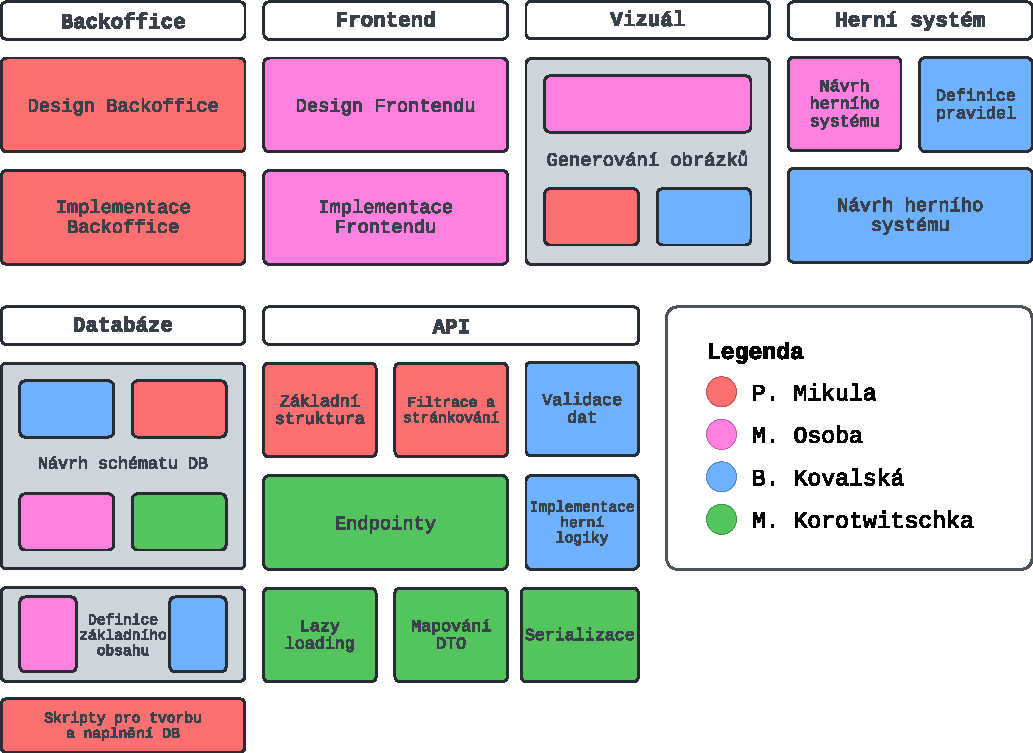
\includegraphics[width=0.95\textwidth]{../../shared/diagrams/blocks}
    \caption{Rozložení práce v týmu}
    \label{fig:job_distribution}
\end{figure}

\subsection{Verzování kódu}
\label{subsec:implementation-collaboration-versioning}
Efektivnost verzování kódu je důležitou součástí každé týmové spolupráce na větším projektu. Pro správu obsahu práce jsem tak využili nástroj Git pod službou GitHub, který nám umožnil efektivně sledovat změny a udržovat si tak přehled o vývoji projektu. Využití Gitu bylo zvoleno především pro jeho jednoduchost a znalost všech členů týmu, kteří s ním již měli zkušenosti v minulosti.

%Pro zajištění správného vývoje byly vytvořeny dvě hlavní větve, které sloužily pro vývoj nových funkcí a opravu chyb. Větve byly následně spojovány pomocí pull requestů, které sloužily pro kontrolu a schválení změn. Tento proces byl zvolen pro zajištění kvality kódu a zamezení chybám, které by mohly vzniknout při nesprávném spojení větví.

\subsubsection*{Větve}
\label{subsubsec:implementation-collaboration-versioning-branches}
V moderních vývojích systému se každá část nebo project celý rozděluje do složitějšího stromu větví známého pod názvem \textit{Git Worfkflow}, jeho efektivní reprezentaci lze vidět na obrázku~\ref{fig:git_workflow}. Tento strom se dělí na 2 hlavní větve, často nazývané \textit{master} a \textit{develop}.

Větev \textit{master} slouží pro produkční verze projektu, které jsou připraveny k nasazení, zatímco větev \textit{develop} slouží pro vývoj nových funkcí. Aktualizace větví tzv. \textit{commits} jsou poté spojovány pomocí pull requestů, které slouží pro kontrolu a schválení změn. Tento proces byl zvolen pro zajištění kvality kódu a zamezení chybám, které by mohly vzniknout při nesprávném spojení větví.

Následně strom obsahuje pod větve vývojové, tyto větve se často štěpí z větve developu a slouží pro vývoj nových funkcí nebo opravu chyb. Po dokončení a úspěšném testování je tato větev spojena zpět do developu a po vydání nové verze je spojena do masteru.

\subsubsection*{Zkratky}
Tabulka zkratek zobrazena v obrázku ~\ref{fig:git_workflow}.

\begin{table}[h]
    \centering
    \resizebox{\textwidth}{!}{%
        \begin{tabular}{l l l}
            \toprule

            \textbf{Příkaz} & \textbf{Zkratka} & \textbf{Význam} \\
            \midrule

            \textbf{git nh} & New Hotfix & Vytvoření větve pro rychlou opravu chyb, která je již v produkci \\
            \textbf{git mh} & Merge Hotfix & Dokončení vývoje a spojení větve zpět do masteru \\
            \textbf{git live} & Release & Publikace nové verze a spojení větve do masteru \\
            \textbf{git nb} & New Bugfix & Vytvoření větve pro opravu chyb, která je ve vývoji \\
            \textbf{git mb} & Merge Bugfix & Dokončení vývoje a spojení větve zpět do developu \\
            \textbf{git uat} & User Acceptance Testing & Vytvoření větve pro testování nové verze \\
            \textbf{git nf} & New Feature & Vytvoření větve pro vývoj nové funkce \\
            \textbf{git mf} & Merge Feature & Dokončení vývoje a spojení větve zpět do developu \\

            \bottomrule
        \end{tabular}}
    \caption{Seznam efektů}
    \label{tab:effects}
\end{table}

%Informace o verzování kódu. Jak se používá Git, jak se vytvářejí větve, jak se dělají pull requesty, jak se řeší konflikty.
%https://www.freecodecamp.org/news/how-to-use-git-best-practices-for-beginners/
%https://stackoverflow.com/questions/19695127/git-workflow-review

\begin{figure}[H]
    \centering
    \includegraphics[width=0.9\textwidth]{figures/GitWorkflow}
    \caption{Ukázka správného použití verzovacího systému Git. \cite{git_workflow}}
    \label{fig:git_workflow}
\end{figure}

\subsection{Sdílení kódu}
\label{subsec:implementation-collaboration-sharing}

\section{Problémy vývoje}
\label{sec:implementation-problems}

\subsection*{Hexagonální grid}
\label{subsec:implementation-problems-hexagon}

%\newpage
%\processDiagram{diagrams/OpenPage}{OpenPage}{0.75\textwidth}{Diagram aaa}
%
%\newpage
%\processDiagram{diagrams/NewObject}{NewObject}{0.75\textwidth}{Diagram průběhu editace nebo přidávání dat}

\endinput